\subsubsection{Auto-regressive Integrated Moving Average}
	Логичным предположением является тот факт, что значения конкретного временного ряда зависят от своих предыдущих значений, как было показано на примере EWMA (\myref{link::ewma}). Обобщая данную мысль, текущее ($t$) значение временного ряда может зависеть от некоторого на $k$ шагов отстающего от него значения ($t - k$). Тогда получается формула вида:
	\begin{equation}
		y_t = \alpha_0 + \sum_{p = 1}^{q} \alpha_p \cdot y_p + \varepsilon_t: \; \varepsilon_t \sim N(0,\sigma^2)
	\end{equation}
	Пока что никаких ограничений на $\alpha_p$ не накладывается. \textbf{Q}: Но что такое переход от $y_t$ элементу ряда к $y_{t - 1}$? \textbf{A}: Это применение некоторого оператора лага (Lag/Backshift) $B: By_t = y_{t - 1}, B^2y_t = y_{t - 2}$ и так далее. \textbf{Q}: Что должен представлять из себя данный оператор? \textbf{A}: 1) Он должен быть линеен, то есть: $B(x_t + k \cdot y_t) = Bx_t + k \cdot By_t = x_{t - 1} + k \cdot y_{t - 1}: k \in \R$. \textbf{Q}: Как грамотно задать данный оператор? \textbf{A}: Представляем ситуацию, в которой необходимо из вектора $Y_n = (y_1, \ldots, y_n)^T$ получить вектор $Y_{n - 1} =  (0, y_1, \ldots, y_{n - 1})^T$, тогда матрица $B: \R^{n \times 1} \to \R^{n \times 1}$ имеет вид.
	\begin{equation}
		\left(\begin{matrix}
			0 & 0 & \cdots & 0\\
			1 & 0 & & 0\\
			\vdots & \ddots & \ddots & \vdots\\
			0 & \cdots & 1 & 0
		\end{matrix}\right) 
		\left(\begin{matrix}
			y_1\\ y_2\\ y_3 \\ \vdots \\ y_n
		\end{matrix}\right) = 
		\left(\begin{matrix}
			0\\ y_1\\ y_2 \\ \vdots \\ y_{n - 1}
		\end{matrix}\right)
	\end{equation}
	Во-первых, она квадратная, во-вторых интересно, что данный оператор является нильпотентным степени $n$. Из этого следует, что a) единственное собственное значение $B$ это $0$ b) $B^n = O$ (нулевая матрица), то есть степень нильпотентности не превосходит $n$. Более подробно в работе \cite{panov_linear_operator}. Но прежде, чем переписать полученную выше сумму в надлежащем виде, вспоминаем о возможной зависимости $y_t$ от предыдущих значений скользящей средней ($\varepsilon_{t - l}$), где $\varepsilon_{t - l}$ - значение, полученное из белого шума \footnote{Белый шум - независимые, взятые из одного распределения величины - часто $N(0,\sigma^2)$.}.
	\begin{equation}
		\begin{split}
			y_t & = \alpha_0 + \sum_{k = 1}^{p} \alpha_k B^k y_{t} + \sum_{j = 1}^{q} \beta_j  B^j \varepsilon_{t} + \varepsilon_t\\
			\left(1 - \sum_{k = 1}^{p} \alpha_k B^k\right) y_t & = \alpha_0 + \left(\sum_{j = 1}^{q} \beta_j B^j\right) \varepsilon_{t}
		\end{split}
	\end{equation}
	При этом $B\alpha_0 = \alpha_0: \alpha_0 \in \R$ по построению. Таким образом, получаем модель авторегрессионной скользящей средней ARMA$(p,q)$. Но по первоначальной предпосылке о стационарности \myref{def::weak_ts_stationarity}, есть желание обобщить модель на случай нестационарных рядов. То есть сделать ее более универсальной. Для этого формально выводим условие стационарности. Выражению $1 - \sum_{k = 1}^{p} \alpha_k B^k$ в соответствие ставим характеристическое уравнение $1 - \sum_{k = 1}^{p} \alpha_k z^k$. Тогда если все корни данного уравнения (в силу Основной теоремы Алгебры, полученный полином над комплексной плоскостью имеет не более, чем $p$ различных корней) $|z_i| > 1$, то данный ряд стационарен. Подробнее для AR(1):
	\begin{equation}
		\begin{split}
			y_t = \alpha \cdot y_{t - 1} + \varepsilon_t \Rightarrow 1 - \alpha \cdot z = 0 \Rightarrow z = \frac{1}{\alpha}\\
			y_{t + 1} - \alpha \cdot y_{t} \approx 0 \Rightarrow \lambda - \alpha = 0 \Rightarrow y_t \approx c \cdot \alpha^t: \; c \in \R 
		\end{split}
	\end{equation}
	Получается, чтобы числовые значения данного ряда не уходили в $\infty$ при $t \to \infty$ необходимо, чтобы в случае AR$(1) \; |z| > 1$, а $|\alpha| < 1$. Аналогично для случаев AR$(p)$. Таким образом, вывод: необходим множитель, который помогал бы последовательности переходить к $d$ - ому порядку интегрирования. \textbf{Q}: Как это сделать? \textbf{A}: $\nabla^1 y_t = y_t - y_{t - 1} = y_t - By_t = (1 - B) y_t, \nabla^2y_t = \nabla^1y_t - \nabla^1 y_{t - 1} = (1 - B) y_t - (1 - B) y_{t - 1} = (1 - B) y_t - (1 - B) By_t = (1 - 2B + B^2) y_t = (1 - B)^2 y_t$ и так далее. Получается, что необходимый множитель: $\nabla^d = (1 - B)^d$. Соответственно формула ARIMA$(p,d,q)$ имеет вид:
	\begin{equation}
		\underbrace{\left(1 - \sum_{k = 1}^{p} \alpha_k \cdot B^k\right) \overbrace{(1 - B)^d}^{\text{I}(d)} y_t}_{\text{AR}(p)} = \overbrace{\alpha_0}^{\text{const}} + \underbrace{\left(\sum_{j = 1}^{q} \beta_j \cdot B^j\right) \varepsilon_{t}}_{\text{MA}(q)}
	\end{equation}
	Получившаяся модель включает в себя авторегрессионную составляющую порядка $p$, скользящую среднюю порядка $q$ и интегрированность порядка $d$. Также стоит отметить, что любой стационарный процесс можно разложить в бесконечный (абсолютно сходящийся) процесс скользящего среднего. Более известен данный факт под названием - разложение Вольда \cite{wold_decomposition}. Для примера предполагаем, что некоторый процесс AR$(1)$ стационарен.
	\begin{equation}
		\begin{split}
			y_t & = \alpha_ 0 + \alpha \cdot y_{t - 1} + \varepsilon_{t}\\
			(1 - \alpha B) \cdot y_t & = \alpha_0 + \varepsilon_{t}\\
			(1 - \alpha B)^{-1}(1 - \alpha B) y_t & = (1 - \alpha B)^{-1} (\alpha_0 + \varepsilon_{t})\\
			y_t & = (1 - \alpha B)^{-1} \cdot \alpha_0 + (1 - \alpha B)^{-1} \cdot \varepsilon_{t}\\
			\text{Но ряд стационарен} \Rightarrow y_t & = \sum_{j = 1}^{\infty} B^j\alpha_0 + \sum_{j = 1}^{\infty} B^j\varepsilon_{t} = \frac{\alpha_0}{1 - \alpha} + \sum_{j = 1}^{\infty} \alpha^j \cdot B^j\varepsilon_{t}
		\end{split}
	\end{equation}
	Более подробно о данной модели написано в \cite{arima}. Процесс обучения (то есть подбора соответствующих коэффициентов модели) происходит посредством применения ММП (Метода Максимального Правдоподобия), максимизирующего вероятность наиболее точно описать входные данные. Глобальная задача, стоящая пред алгоритмом подбора параметров (читать далее - алгоритма обучения) это:
	\begin{equation}
		\sum_{p}^n e_p^2 \to \min_{\alpha \in \R^p, \; \beta \in \R^q}
	\end{equation}
	Где $e_p = y_p - \hat{y}_p$ - остаток (разница между предсказанным и исходным значением). Это очень похоже на Метода Наименьших Квадратов (МНК), только МНК дает аналитическую формулу оценок коэффициентов, а в общем случае это не всегда возможно, поэтому для подобных задач часто применяется ММП. Тут же встает вопрос: \textbf{Q}: Как понять, какая модель лучше описывает данные? \textbf{A}: 1) Критерий Акаике (AIC):
	\begin{equation}
		J_{\text{AIC}} = 2k + n \cdot \ln\left[\frac{1}{n} \sum_{p = 1}^n \left(y_p- \hat{y}_p \right)^2\right]
	\end{equation}
	Где $k$ - количество параметров в обучаемой модели, $n$ - общее количество наблюдений, $(y_p - \hat{y}_p)^2 = e_p^2$ - остаток от регрессии 2) Байесовский информационный критерий (BIC):
	\begin{equation}
	 J_{\text{BIC}} = \frac{1}{n} \sum_{p = 1}^n \left(y_p - \hat{y}_p \right)^2 + \frac{k \hat{\sigma}^2 \ln(n)}{n}
	\end{equation} 
	Где $\hat{\sigma}^2$ - оценка (так как реальное значение неизвестно) дисперсии шума ряда, полученного по формуле $(y - \hat{y})$. \cite{alexandridis2014wavelet} \textbf{Q}: Однако тут появляется еще один вопрос: как человеку понять, какой порядок AR($\cdot$) и MA($\cdot$) должен быть? \textbf{A}: Существует 2 способа, чтобы выяснить это. ACF$(k)$ (Auto Correlation Function) и PACF$(k)$ (Partial Auto Correlation Function). Как видно из названия - это некоторые функции от переменной $k$. \textbf{Q}: Что они характеризуют? \textbf{A}: 1) ACF - основанная на конкретном наборе данных дискретная функция, вычисляемая на основе формулы: 
	\begin{equation}
		\text{ACF}(k) = \hat{\rho}_k = \hat{\text{corr}}(y_t, y_{t - k})
	\end{equation}
	2) PACF - частная автокорреляционная функция. Вычисляется на основе оцененной модели AR$(k)$. Строится график коэффициентов при лагах. В итоге формула функции приобретает вид:
	\begin{equation}
		\text{PACF}(k) = \hat{\alpha}_k
	\end{equation}
	Как было сделано для предыдущей модели, иллюстрируем вышеизложенную теорию на примере. Рассматриваем цены открытия акций компании Apple за 2021 год. Стоит заранее сказать, что прежде, чем обучить модель, проверяем сам ряд на стационарность, то есть - на наличие корней $|z_j| < 1$, что свидетельствует о нестационарности исследуемого ряда.
	\begin{itemize}
		\item В настоящем исследовании проверка стационарности временного ряда проводится посредством применения Аугментированного теста Dickey–Fuller (ADF) \cite{adf_unit_root_test}, а также Kwiatkowski–Phillips–Schmidt–Shin (KPSS) \cite{kpss_unit_root_test}. Для ADF \textbf{H0} - нестационарность (простая незначимость переменной), то есть наличие единичного корня, а для KPSS \textbf{H0} - стационарность ряда.
		\begin{table}[H]
			\centering
			\begin{tabular}{r|cc}
				\toprule
				& ADF & KPSS\\
				\midrule[0.02cm]
				Статистика & $0.017$ & $1.802$\\
				P-val & $0.96$ & $< 0.01$\\
				Критическое значение ($1\%$) & $-3.457$ & $0.739$\\
				Критическое значение ($5\%$) & $-2.873$ & $0.463$\\
				Критическое значение ($10\%$) & $-2.573$ & $0.347$\\
				\midrule[0.02cm]
			\end{tabular}
			\caption{Тестирование исходного ряда на стационарность}
		\end{table}
		Следовательно, ряд не является стационарным. Таким образом, переходим к первым разностям и проводим повторное тестирование.
		\begin{table}[H]
			\centering
			\begin{tabular}{r|cc}
				\toprule
				& ADF & KPSS\\
				\midrule[0.02cm]
				Статистика & $-17.740$ & $0.239$\\
				P-val & $0.00$ & $\gg 0.10$\\
				Критическое значение ($1\%$) & $-3.457$ & $0.739$\\
				Критическое значение ($5\%$) & $-2.873$ & $0.463$\\
				Критическое значение ($10\%$) & $-2.573$ & $0.347$\\
				\midrule[0.02cm]
			\end{tabular}
			\caption{Тестирование первых разностей на стационарность}
		\end{table}
	
		\item Далее строим ACF и PACF, чтобы выяснить порядок авторегрессии и скользящей средней. Делать это уже имеем право, так как полученный процесс является стационарным.
		\begin{figure}[H]
			\centering
			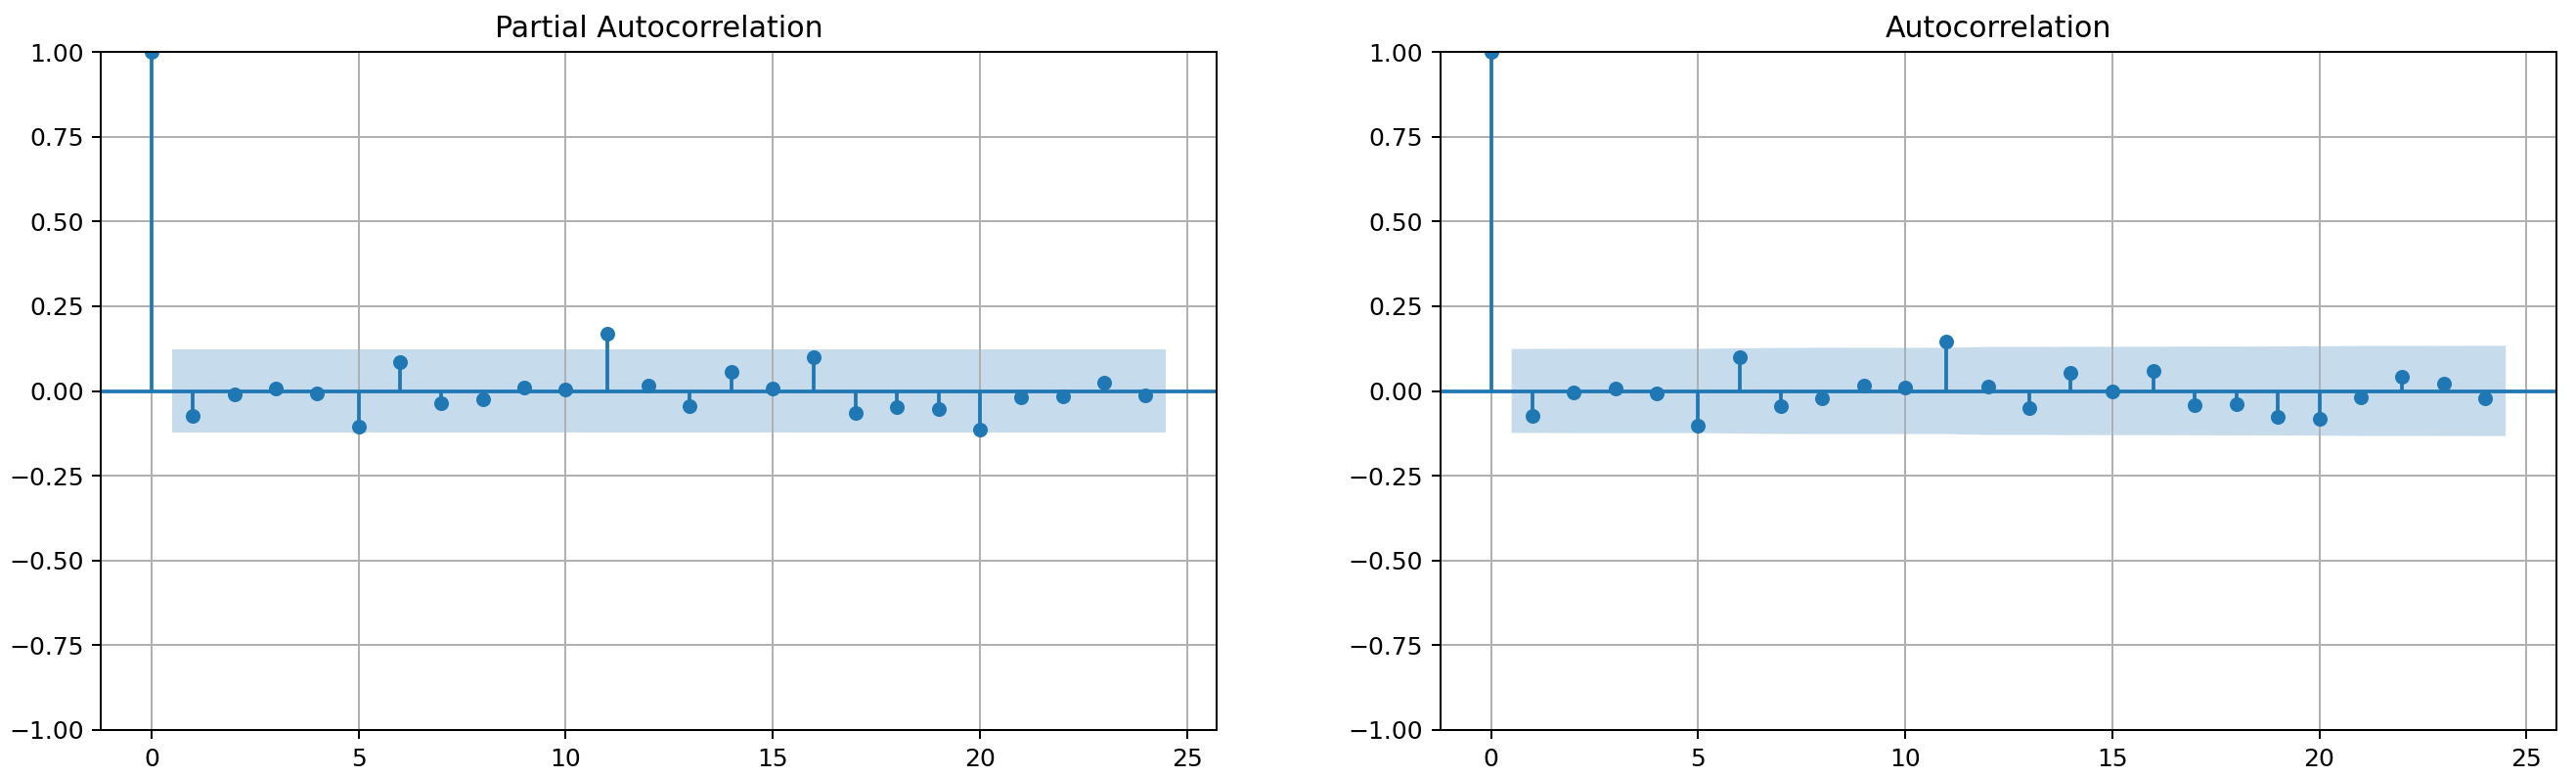
\includegraphics[width=17cm, height=5cm]{arima/initial_acf_pacf.png}
			\caption{ACF и PACF для $\nabla^1y_t$}
		\end{figure}
		В данном случае получаем, что лучшим вариантом модели является случайное блуждание. Модель вида  - пример для Random Walk$(k)$, впервые разработанная Луи Башелье \cite{fama_market_efficiency} в 1900 году в работе, посвященной анализу фондового рынка:
		\begin{equation}
			y_t = \alpha_0 + \sum_{p = 1}^k y_{t - p} + \varepsilon_{t}
		\end{equation}
		То есть формальная запись модели, которую мы оцениваем далее - это ARIMA(0, 1, 0). Так как ни скользящей средней, ни автокорреляции не было выявлено для 1-ой разности.
		
		\item Получаем сводную таблицу о качестве полученной модели:
		\begin{table}[H]
			\centering
			\begin{tabular}{r|ccc}
				\toprule
				Модель & \multicolumn{3}{c}{ARIMA$(0, 1, 0)$}\\
				\midrule[0.02cm]
				Зависимая переменная & \multicolumn{3}{c}{Цена открытия}\\
				Количество наблюдений & \multicolumn{3}{c}{222} \\
				AIC & \multicolumn{3}{c}{$934.71$} \\
				BIC & \multicolumn{3}{c}{$941.56$} \\
				\midrule[0.02cm]
				Тест Ljung-Box (Q) & \multicolumn{2}{c}{$0.04$} & P-val ($0.83$)\\
				Тест Jarque-Bera (JB) & \multicolumn{2}{c}{$6.50$} & P-val ($0.04$)\\
				Тест Heteroskedasticity & \multicolumn{2}{c}{$0.51$} & P-val ($0.00$)\\
				\midrule[0.02cm]
				Константа - $\alpha_0$ & $0.079$ & std (0.135) & P-val (0.557)\\
				Оцененная дисперсия - $\sigma^2$ & $3.949$ & std (0.324) & P-val (0.000)\\
				\midrule[0.02cm]
			\end{tabular}
			\caption{Таблица по оценке иллюстративной модели ARIMA$(0,1,0)$}
		\end{table}
		Тест Ljung-Box \cite{ljung_box_test} - проверка на наличие автокорреляции в остатках. \textbf{H0}: автокорреляции в остатках нет, то есть получен белый шум. Тест Jarque-Bera \cite{jarque_bera_test}- тест на нормальность, где \textbf{H0}: нормальность входных на тест данных. Однако в данном случае присутствует гетероскедастичность, которую можно убрать посредством применения скорректированной ковариационной матрицы HAC \cite{hac_standard_errors}, однако в текущем случае необходим лишь пример модели, а не идеальная ее версия, поэтому оставляем ситуацию с ошибками модели как есть и исследуем остатки регрессии.
		\item В графическом варианте остатки регрессии представляются как некоторый процесс (без тестов не можем сказать, какой именно), а также плотность распределения данного числового ряда.
		\begin{figure}[H]
			\centering
			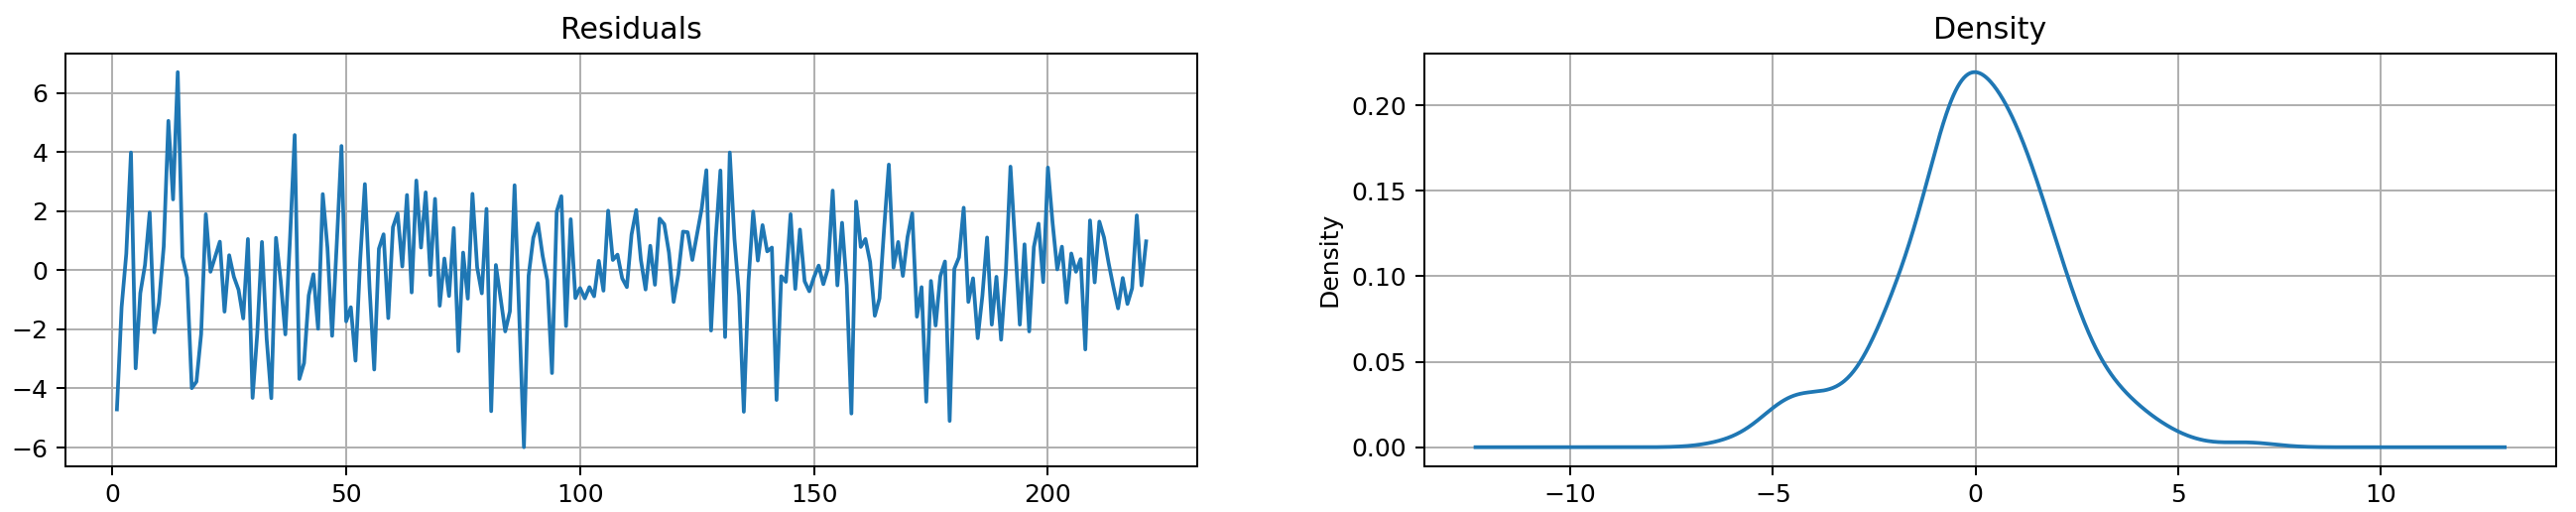
\includegraphics[width=17cm, height=4cm]{arima/residuals_and_density.png}
			\caption{Остатки и распределение остатков моделирования RW}
		\end{figure}
		Исходя из визуального анализа, распределение похоже на нормальное, более того формальные показатели, а именно тесты Ljung-Box и Jarque-Bera, также подтверждают данное предположение. Отсюда вывод, модель подобрана корректно, более ничего необъясненного в данных не осталось. Остался только белый шум. Однако также проверяем: есть ли в остатках модели автокорреляция.
		
		\item Основываясь на графиках ACF и PACF, вывод: автокорреляции в остатках нет.
		\begin{figure}[H]
			\centering
			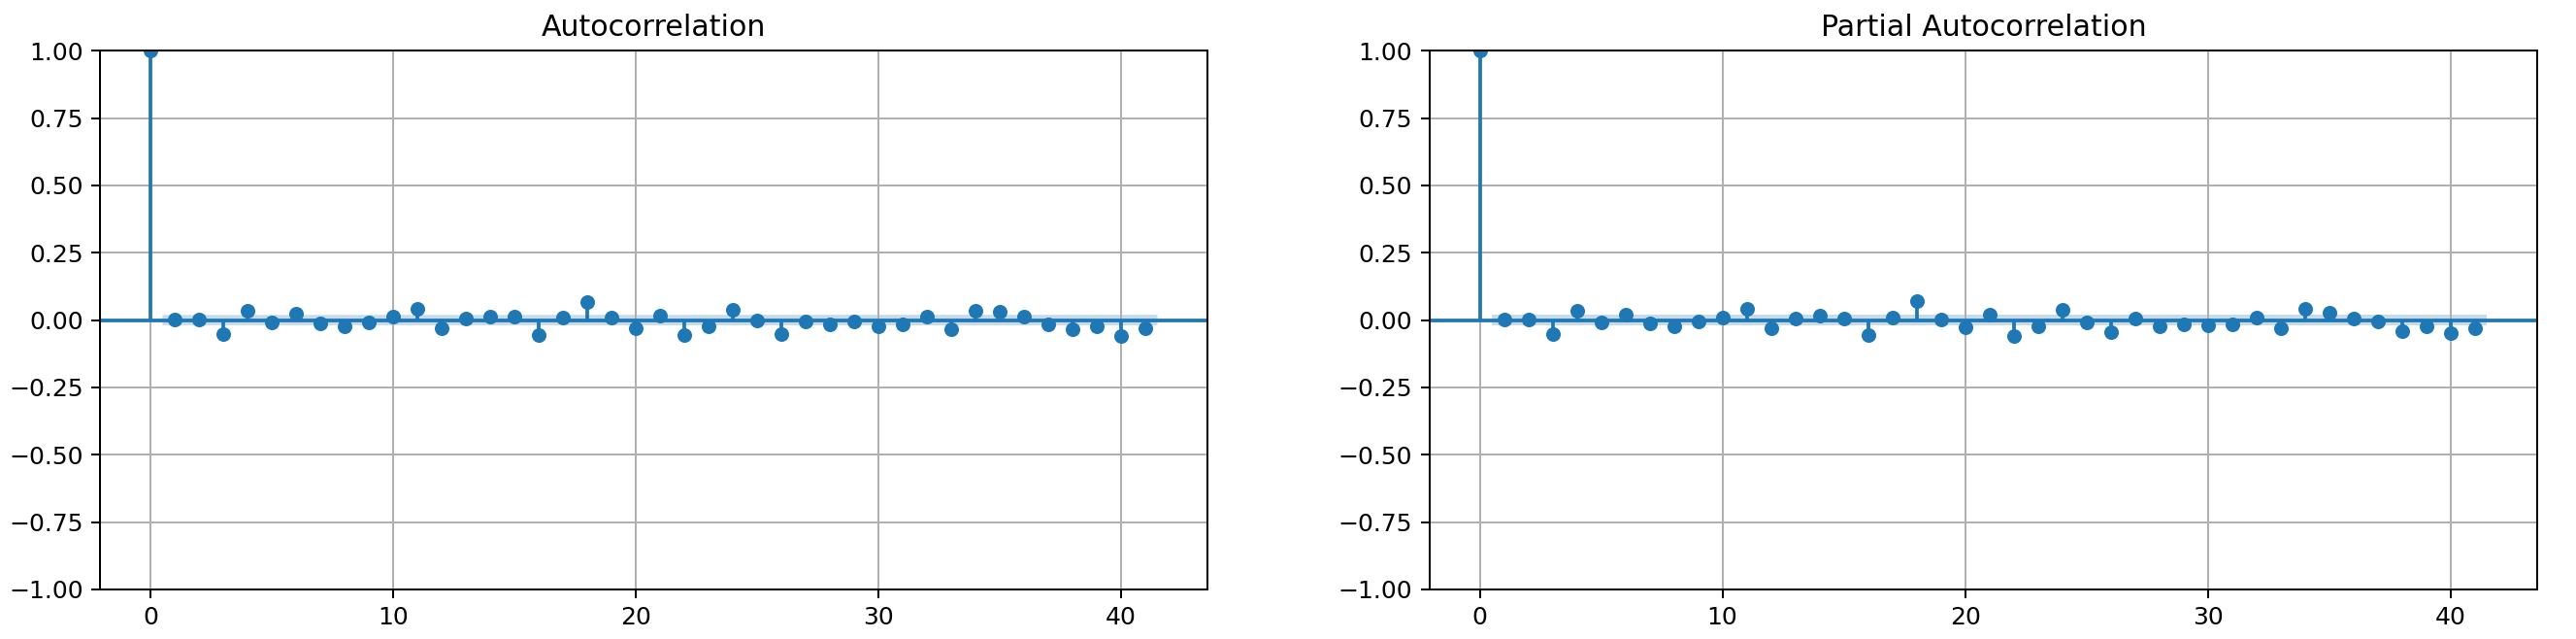
\includegraphics[width=17cm, height=4cm]{arima/residuals_acf_pacf.png}
			\caption{ACF и PACF для остатков моделирования RW}
		\end{figure}
	
		\item Несмотря на информативность уже изображенных графиков, главной ценностью настоящей модели является способность к предсказанию.
		\begin{figure}[H]
			\centering
			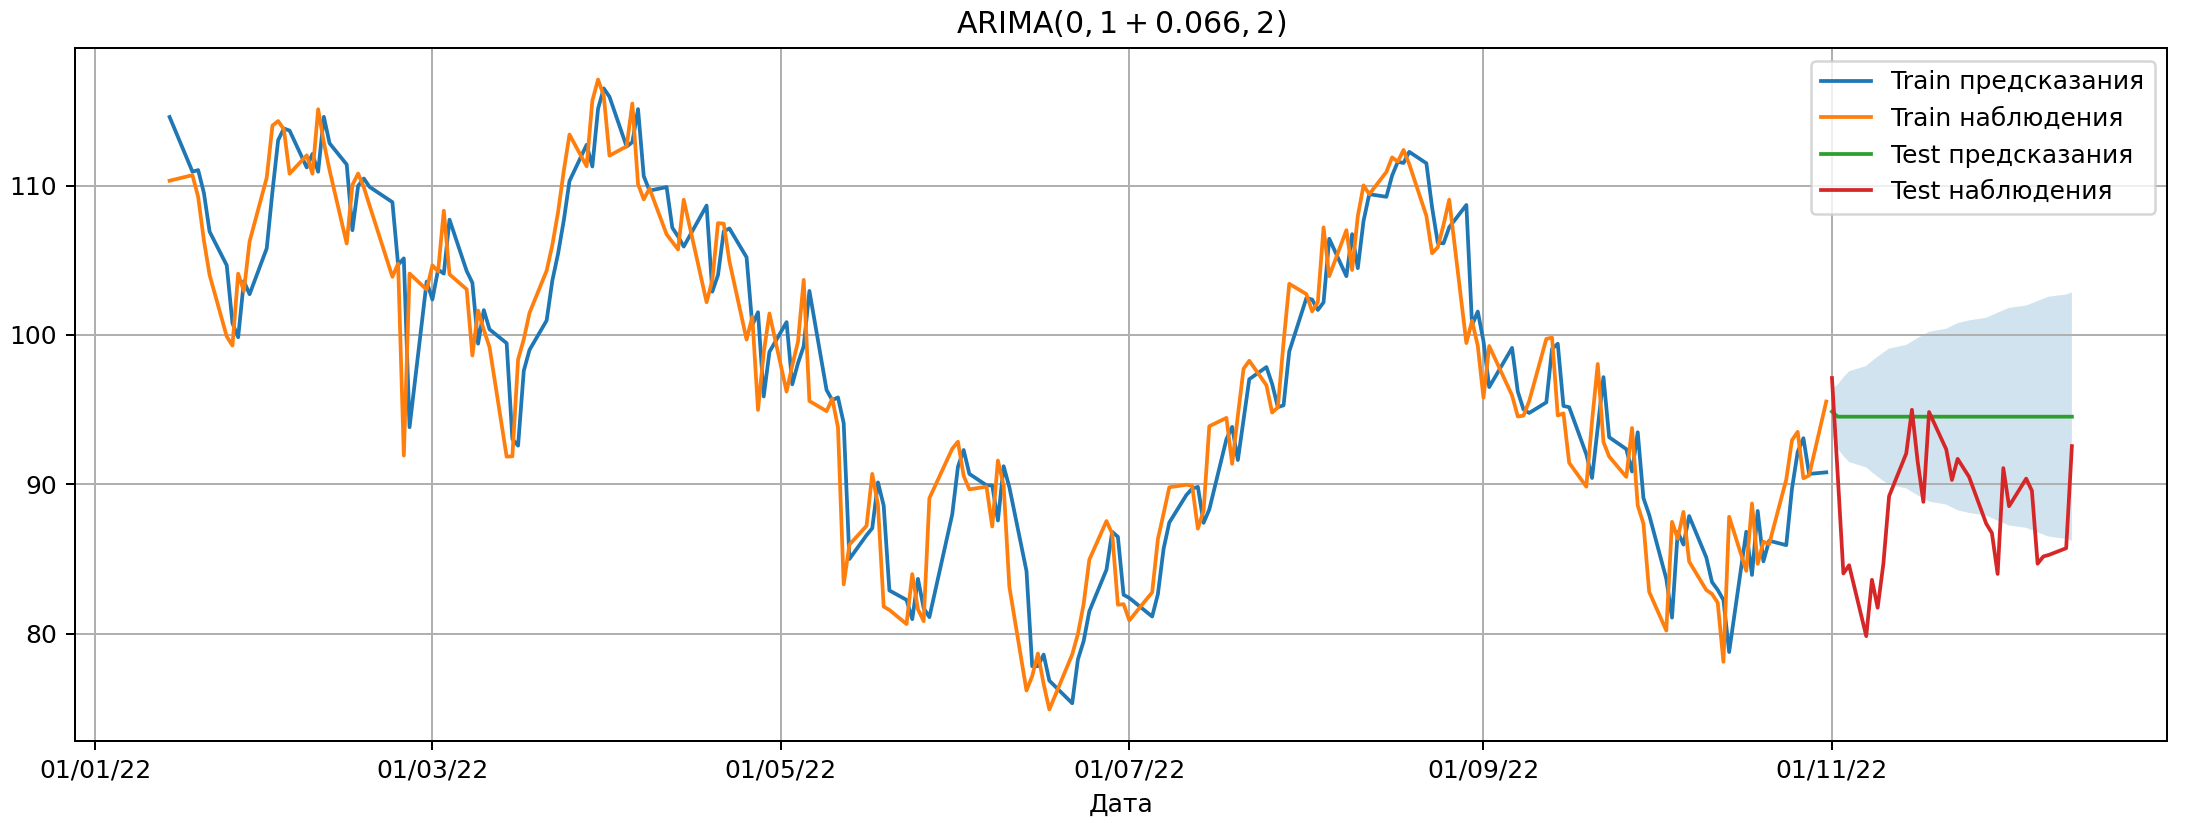
\includegraphics[width=17cm, height=6.25cm]{arima/final_picture.png}
			\caption{Моделирование предсказаний посредством модели RW}
		\end{figure}
	\end{itemize}
	\noindent Здесь синим цветом выделяется доверительный интервал для уровня значимости $5\%$. Причем интересно, что в доверительный интервал почти не попадают реальный значения, что говорит о больших трудностях как для описания данных, так и для предсказания посредством Random Walk. Train/Test - это дробление выборки на обучающие данные (на которых подбираются коэффициенты) и тестовые (на которых проводится проверка адекватности предсказаний модели). Если подобного дробления не проводить, то возможно переобучение, откуда получаем нулевую точность предсказания. Отсюда вывод, что для получения большей точности необходим поиск иного рода моделей. Но, как только что было сказано, с помощью данной модели можно предсказывать последующие значения числовой последовательности, опираясь на исходные показатели временного ряда, поэтому данная модель также включается в список сравнительной таблицы. 
	